\documentclass[tikz]{standalone}
\usetikzlibrary{positioning}

\begin{document}
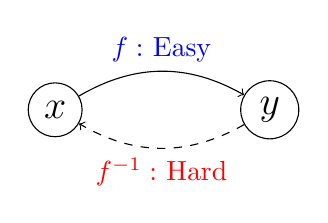
\begin{tikzpicture}[s/.style = {draw, circle, minimum size = 12pt, font = \Large}]
  \node (x) [s] {$x$};
  \node (y) [s, right = 2.0cm of x] {$y$};

  \draw [bend left, ->] (x) to node [above] {\textcolor{blue}{$f:$ Easy}} (y);
  \draw [bend left, ->, dashed] (y) to node [below] {\textcolor{red}{$f^{-1}:$ Hard}} (x);
\end{tikzpicture}
\end{document}
